\documentclass[a4paper, 11pt]{article}
\usepackage{comment}
\usepackage{lipsum} 
\usepackage{fullpage} %cambiar margen
\usepackage[a4paper, total={7in, 10in}]{geometry}

\usepackage{amssymb,amsthm} 
\usepackage{amsmath}
\newtheorem{theorem}{Theorem}
\newtheorem{corollary}{Corollary}
\usepackage{graphicx}
\usepackage{tikz}
\usetikzlibrary{arrows}
\usepackage{verbatim}
%\usepackage[numbered]{mcode}
\usepackage{float}
\usepackage{tikz}
\usetikzlibrary{shapes,arrows}
\usetikzlibrary{arrows,calc,positioning}
\usepackage{mathpazo} %tipo de letra 
\usepackage[utf8]{inputenc} %codificación
\usepackage[T1]{fontenc} %digitación de tildes y ñ
\usepackage[spanish]{babel} %paquete de soporte español

\tikzset{
	block/.style = {draw, rectangle,
		minimum height=1cm,
		minimum width=1.5cm},
	input/.style = {coordinate,node distance=1cm},
	output/.style = {coordinate,node distance=4cm},
	arrow/.style={draw, -latex,node distance=2cm},
	pinstyle/.style = {pin edge={latex-, black,node distance=2cm}},
	sum/.style = {draw, circle, node distance=1cm},
}
\usepackage{xcolor}
\usepackage{mdframed}
\usepackage[shortlabels]{enumitem}
\usepackage{indentfirst}
\usepackage{hyperref}

\usepackage{listings}
\lstset{literate=
  {á}{{\'a}}1
  {é}{{\'e}}1
  {í}{{\'i}}1
  {ó}{{\'o}}1
  {ú}{{\'u}}1
  {Á}{{\'A}}1
  {É}{{\'E}}1
  {Í}{{\'I}}1
  {Ó}{{\'O}}1
  {Ú}{{\'U}}1
  {ñ}{{\~n}}1
  {ü}{{\"u}}1
  {Ü}{{\"U}}1
}

\lstdefinestyle{customc}{
  belowcaptionskip=1\baselineskip,
  breaklines=true,
  frame=L,
  xleftmargin=\parindent,
  language=Python,
  showstringspaces=false,
  basicstyle=\footnotesize\ttfamily,
  keywordstyle=\bfseries\color{green!40!black},
  commentstyle=\itshape\color{purple!40!black},
  identifierstyle=\color{blue},
  stringstyle=\color{orange},
}

\lstdefinestyle{customasm}{
  belowcaptionskip=1\baselineskip,
  frame=L,
  xleftmargin=\parindent,
  language=[x86masm]Assembler,
  basicstyle=\footnotesize\ttfamily,
  commentstyle=\itshape\color{purple!40!black},
}

\lstset{escapechar=@,style=customc}



\renewcommand{\thesubsection}{\thesection.\alph{subsection}}

\newenvironment{problem}[2][Ejercicio]
{ \begin{mdframed}[backgroundcolor= red!50] \textbf{#1 #2} \\}
	{  \end{mdframed}}

% Define solution environment
\newenvironment{solution}
{\textcolor{blue}{\textbf{\textit{Solución:\\\noindent}}}}


\renewcommand{\qed}{\quad\qedsymbol}

% \\	
\begin{document}
	\noindent
	%%%%%%%%%%%%%%%%%%%%%%%%%%%%%%%%%%%%
	
	\begin{minipage}[b][1.2cm][t]{0.8\textwidth}
		\large\textbf{César Isaí García Cornejo} \hfill \textbf{Tarea 5}  \\
		cesar.cornejo@cimat.mx \hfill \\
		\normalsize Computo Científico \hfill Semestre 3\\
	\end{minipage}
	
	\hspace{14.4cm}
	\begin{minipage}[b][0.03cm][t]{0.12\linewidth}
		
		\vspace{-2.2cm}
		%%%La Ruta dependera de donde este alojado el main y la imagen
		
\includegraphics[scale=0.3]{Figures/EscudoCimat.png}
	\end{minipage}
	
	\noindent\rule{7in}{2.8pt}
	
	%%%%%%%%%%%%%%%%%%%%%
	%%%%%%%%%%%%%%%%%%%%%%%%%%%%%%%%%%%%%%%%%%%%%%%%%%%%%%%%%%%%%%%%%%%%%%%%%%%%%%%%%%%%%%%%%%%%%%%%%%%%%%%%%%%%%%%%%%%
	% Problem 1
	%%%%%%%%%%%%%%%%%%%%%%%%%%%%%%%%%%%%%%%%%%%%%%%%%%%%%%%%%%%%%%%%%%%%%%%%%%%%%%%%%%%%%%%%%%%%%%%%%%%%%%%%%%%%%%%%%%%%%%%%%%%%%%%%%%%%%%%%
	\setlength{\parskip}{\medskipamount}
	\setlength{\parindent}{0pt}
%/////////// Ejercicio 1 /////////////////

\begin{problem}{1}
    Definir la cdf inversa generalizada $F_X^{-1}$ y demostrar que en el caso de variables aleatorias continuas esta coincide con la inversa usual. Demostrar además que en general para simular de $X$ podemos simular $u\sim U(0,1)$ y $F_X^{-}(u)$ se distribuye como $X$. 
\end{problem}

\begin{solution} 
    Definimos la inversa generalizada de la variable aleatoria $X$ como la función
    \begin{align*}
        F^{-}_X(t) = inf\{x\in \mathbb{R}:F_X(x)\geq t \}.
    \end{align*}
    Para variables aleatorias continuas sabemos que $F_X(x)$ es una función monótona creciente en el soporte de $X$. Es decir, tomemos $x,y \in supp(X)$, entonces $x<y$ si y solo si
    \begin{align*}
        F_X(x) < F_X(y)
    \end{align*}
    donde $F(x)$ es una función biyectiva. Luego, existe su función inversa denotada por $F_X^{-1}(t)$.
    Entonces, usando la invertivilidad de la función de distribución en la definición de inversa generalizada
    \begin{align*}
        F^{-}_X(t) &= inf\{x\in \mathbb{R}:F_X(x)\geq t \},\\
            &= inf\{ x\in \mathbb{R}:x \geq F_X^{-1}(t) \}
    \end{align*}
    como $F_X$ es continua existe $x_0$ tal que $F_X(x_0) = t$, es decir $x_0 = F^{-1}_X(t)$. Luego, por la monotonía se sigue que el ínfimo se alcanza y
    \begin{align*}
        F^{-}_X(t) = F^{-1}_X(t)
    \end{align*}
    que nos muestra que para variables $X$ continuas su inversa coincide con la inversa generalizada.

    Para la segunda demostración, primeramente probaremos lo siguiente. Sea $X$ una variable aleatoria continua y $F_X$ su función de distribución, entonces la variable aleatoria $Y = F_X(X)$ tiene distribución uniforme en el intervalo (0,1).

    Para probarlo, es inmediato
    \begin{align*}
        \mathbb{P}\left (Y\leq y   \right ) = \mathbb{P}\left (F_X(X) \leq y \right ) = \left\{\begin{matrix}
            0 & y < 0 \:\:\:o\:\:  y = 0 \:\: y \:\: F_X(x)>0 \:\: \:\: \forall x \\
            1 & y \geq 1 
            \end{matrix}\right.
    \end{align*}
    Por otra parte, si $y \in (0,1)$ o $y=0$ y $F_X(x) =0$ para alguna $x$, definamos: 
    \begin{align*}
        x_0 = \text{sup}\{x \in \mathbb{R}: F_X(x) = y \}
    \end{align*}
    Como $F_X$ es continua, se tiene $F_X(x_0) = y$. Además $F_X(x) > y $ para cualquier $x > x_0$ y $F_X(x) \leq y$ para cualquier $x < x_0$. Es decir, $F_X(x) \leq y$ si y sólo si $x\leq x_0$. Por tanto
    \begin{align*}
        \mathbb{P}\left (F_X(X) \leq y  \right ) = \mathbb{P}\left (X \leq x_0  \right ) = F_X(x_0) = y.
    \end{align*}
    Así que
    \begin{align*}
        \mathbb{P}\left (Y\leq y  \right ) = \mathbb{P}\left (F_X(X) \leq y \right ) = \left\{\begin{matrix}
            0 & y < 0  \\
            y & y\in(0,1)\\
            1 & y \geq 1 
            \end{matrix}\right.
    \end{align*}
    que es la distribución de la variable aleatoria uniforme en el intervalo (0,1).
    Para mostrar el segundo enunciado del Ejercicio 1, usaremos el resultado previo definiendo $X = F^{-1}_X(Y)$. Usando la invertivilidad $F_X(X) = Y$ en el cálculo con $Y\sim$Unif(0,1), es directo
    \begin{align*}
        F_X(q) = \mathbb{P}\left (X \leq q  \right ) = \mathbb{P}\left (F(X) \leq F(q)  \right ) = \mathbb{P}\left (Y \leq F(q)   \right ) = F(q)
    \end{align*}
    para $q \in (0,1)$. Entonces $X$ tiene como función de distribución $F_X$, que es lo que se quería probar.
\end{solution}


\begin{problem}{2}
    Implementar el siguiente algoritmo para simular variables aleatoria uniformes:
    \begin{align*}
        x_i = 107374182 x_{i-1} + 104420 x_{i-5} \:\:\:\: \text{mod } 2^{31} - 1
    \end{align*}
    regresa $x_i$ y recorrer el estado, esto es $x_{j-1} = x_j$; $j=1,2,3,4,5$; ?` Parecen $U(0,1)$? 
\end{problem}

\begin{solution} 
    Para la implementación se creo una función llamada uniforme que toma dos argumentos, $n$ es la cantidad de valores que toma de la recursión de congruencia. El segundo argumento es la semilla, si no se ingresa nada, la semilla predeterminada será dada por el tiempo del computador que nos permite acceder la librería time. Con la semilla determinada, se da un vector de valores arbitrarios para ser el vector inicial.

    Posterior a los cinco valores iniciales, tomamos un vector $X_t$ de tamaño $n$ que nos da la recursión dada pero reescalamos cada valor entre el valor máximo, que es $2^{31}-2$, para tener valores acotados entre cero y uno. Consideremos $n = 100$ y tomemos un histograma 
    \begin{figure}[H] 
        \centering 
        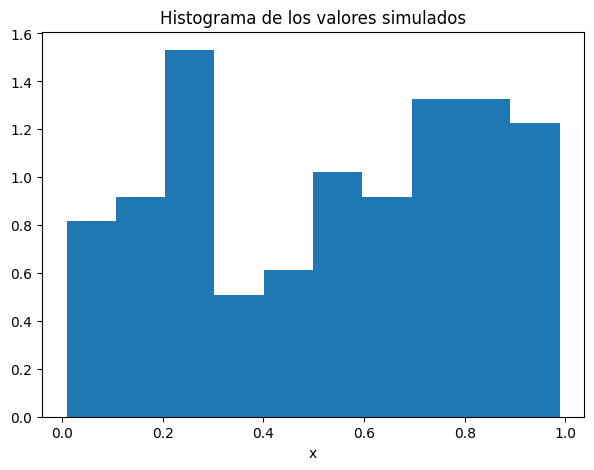
\includegraphics[width = 10cm]{Figures/histo1.png}               
        \caption{Histograma del generador de congruencia lineal $n = 100$.}
        \label{Fig. 2.01}
    \end{figure} 

    \begin{figure}[H] 
        \centering 
        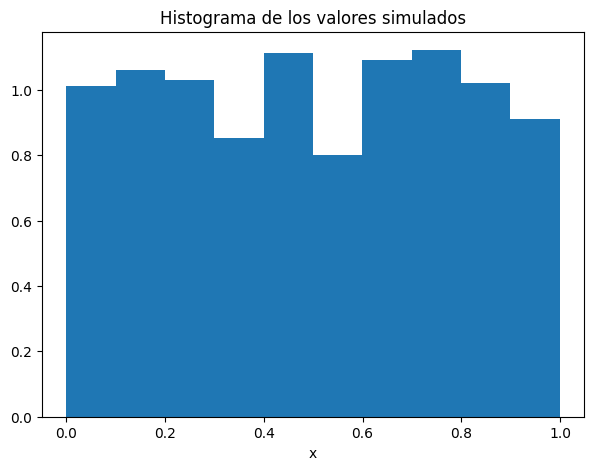
\includegraphics[width = 10cm]{Figures/histo2.png} 
        \caption{Histograma del generador de congruencia lineal $n=1000$.}
        \label{Fig. 2.02}
    \end{figure} 

    \begin{figure}[H] 
        \centering 
        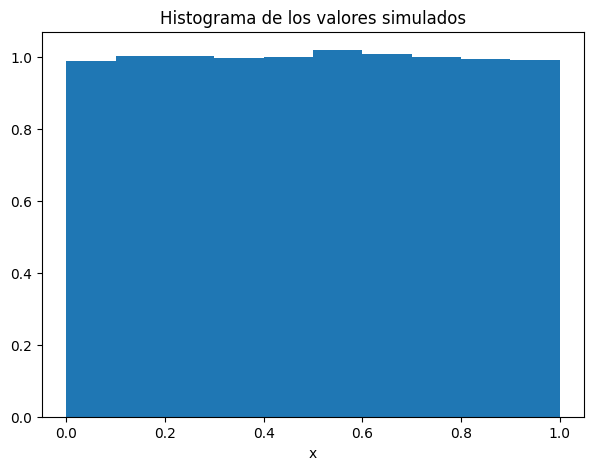
\includegraphics[width = 10 cm]{Figures/histo3.png} 
        \caption{Histograma del generador de congruencia lineal $n = 100000$.}
        \label{Fig. 2.03}
    \end{figure} 

    Podemos ver que parece converger a una distribución uniforme en (0,1). En el código se hace la comparación de este generador con el de scipy. Ambos histogramas tienen comportamientos similares. No podemos afirmar que distribuyen uniforme, sin embargo no tenemos evidencia de que no lo sea. Para poder concluir se requiere de una prueba de ajuste de bondad, sin embargo no es objetivo del ejercicio. Entonces, por lo visto en los histogramas podemos pensar que estamos simulando variables aleatorias uniformes.



\end{solution}



\newpage


\begin{problem}{3}
    ?` Cuál es el algoritmo que usa \textit{scipy.stats.uniform} para generar números aleatorios? ?`Cómo se pone la semilla? ?`y en R?
\end{problem}

\begin{problem}{4}
    ?` En \textit{scipy} que funciones hay para simular un variable aleatoria genérica discreta? ?` tienen preprocesos?
\end{problem}

\begin{problem}{5}
    Implementar el algoritmo Adaptative Rejection Sampling y simular de una $Gama(2,1)$ 10,000 muestras. ?` cuando es conveniente dejar de adaptar la envolvente? (vea alg. A.7, p 54 Robert y Casella, 2da ed.)
\end{problem}

\begin{solution} 
    Se nos pide usar el método Adaptive Rejection Sampling para simular de una Gamma(2,1) con función de densidad
    \begin{align*}
        f(x) = xe^{-x}
    \end{align*}
    Cómo el cuantil del 95\% es menor que 5, entonces la distribución cae rápidamente a cero para valores posteriores.
    Consideramos la aproximación del techo para un dominio de [0.01, 8] donde cada extremos son los valores mínimo y máximo de la rejilla inicial
    \begin{figure}[H] 
        \centering 
        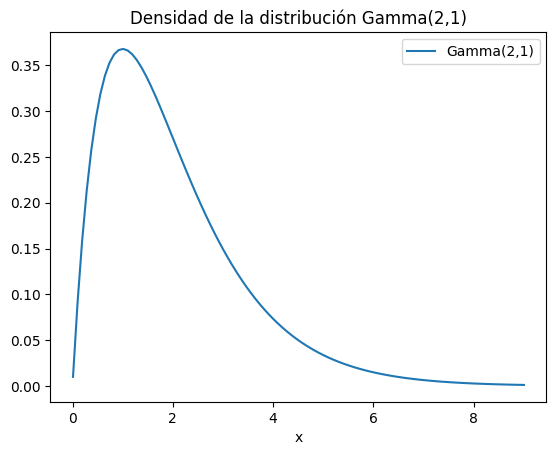
\includegraphics[width = 11 cm]{Figures/DistGamma.png} 
        \caption{Densidad de la distribución gamma(2,1) para simulación}
        \label{Fig.5.01}
    \end{figure} 

    Calculamos la log-densidad. Como vemos que es cóncava, entonces la distribución Gamma(2,1) pertenece a la familia de las distribuciones log-cóncavas. Entonces, se cumple una de las hipótesis del método ARS. Empecemos por establecer una rejilla inicial de 5 valores. En esta rejilla es necesario obtener una función h(x) tal que
    \begin{align*}
        \log f(x) \leq h(x)
    \end{align*}
    para todo $x \in supp(f(x))$.
    Tal \textit{envolvente} dada por el método ARS es tal que, para cada valor de la rejilla, se obtienen en términos de los segmentos de las rectas creadas por puntos adyacentes. 

    Por dar un ejemplo, consideremos la rejilla X = [0.4,1,3,8]
    entonces, evaluamos cada punto en la rejilla en la log-densidad. Obtenemos la siguiente figura
    \begin{figure}[H] 
        \centering 
        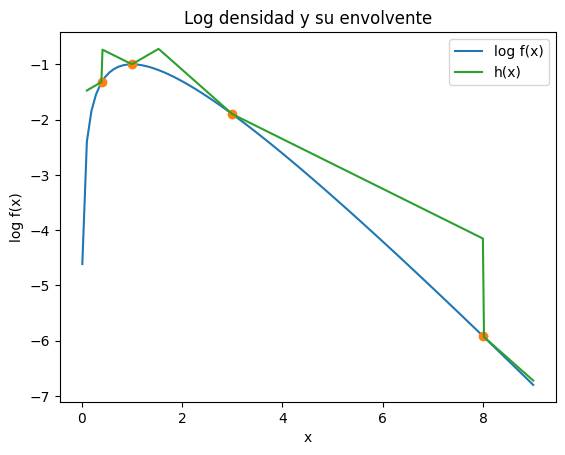
\includegraphics[width = 11 cm ]{Figures/LogDist.png} 
        \caption{Log f(x) para la distribución Gamma(2,1) y la envolvente construida con la rejilla inicial dada.}
        \label{Fig. 5.02}
    \end{figure} 

    Con la envolvente calculada, podemos regresar a la distribución Gamma, sin logaritmos, al igual que a la envolvente, donde vemos que dicha envolvente es una mezcla de exponenciales. 
    \begin{figure}[H] 
        \centering 
        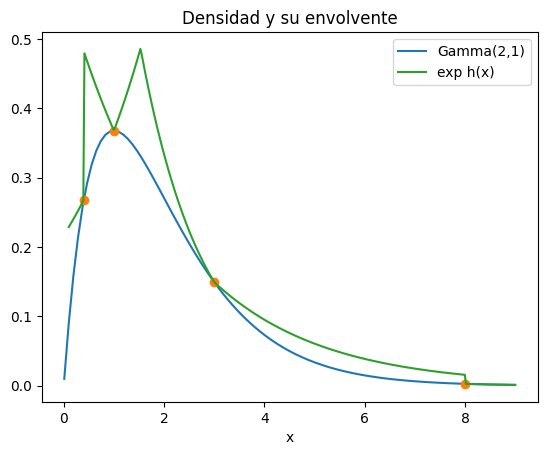
\includegraphics[width = 11 cm ]{Figures/DistEnvol.png} 
        \caption{Función de densidad de la Gamma(2,1) y su envolvente}
        \label{Fig. 5.03}
    \end{figure} 

    Posteriormente, es necesario simular de la función techo $g(x) = \exp(h(x))$. Para ello usamos el resultado del inciso 1. Es decir, generamos una función acumulada de probabilidad para $g(x)$ con esto tenemos que crear ahora la función para la inversa generalizada dada un $u\in [0,1]$. Simulando la variable aleatoria uniforme $u$ y evaluando en la inversa generalizada $ z = g^{-}(u)$ tenemos una simulación de la densidad techo.

    Ahora usando el método de accept-reject. Tomamos la simulación $z$ y una nueva simulación de la uniforme $u$ y aceptamos como muestras de la función de densidad $f$ solo para aquellas muestras $z$ que satisgan que $u *f(z) < g(z)$. En caso de no aceptar se rechaza la muestra y se actualiza con la función constructor() para una nueva rejilla donde se agrega el simulado en la rejilla. Es decir, se vuelve a hacer el mismo procedimiento para simular de la función envolvente $g$ actualizada.  


    La actualización de la rejilla tras rechazar ciertas muestras nos actualiza la envolvente. En este caso, se decidio tomar solo una cantidad fija de actualizaciones ya que es computacionalmente pesado actulizar arbitrariamente. Para cuatro actualizaciones tenemos que la envolvente en la log-densidad es
    \begin{figure}[H] 
        \centering 
        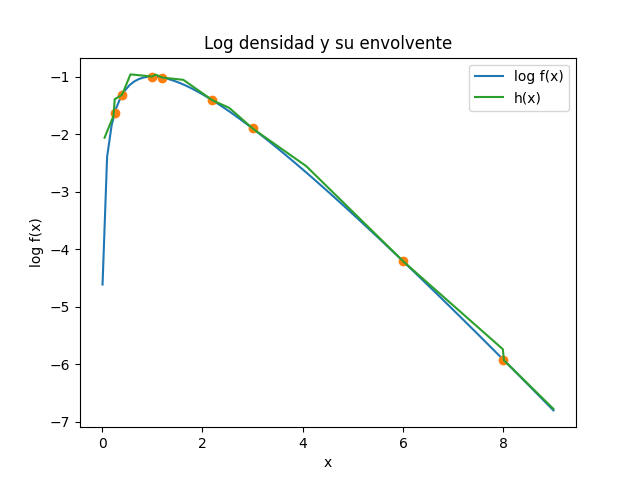
\includegraphics[width = 11 cm ]{Figures/EnvolModificada.png} 
        \caption{Envolvente modificada con más puntos en la rejilla}
        \label{Fig. 5.04 }
    \end{figure} 

    Ya con la envolvente modificada, se toman ahora las simulaciones de 100000 elementos y se grafican en un histograma junto a la densidad gamma(2,1).

    \begin{figure}[H] 
        \centering 
        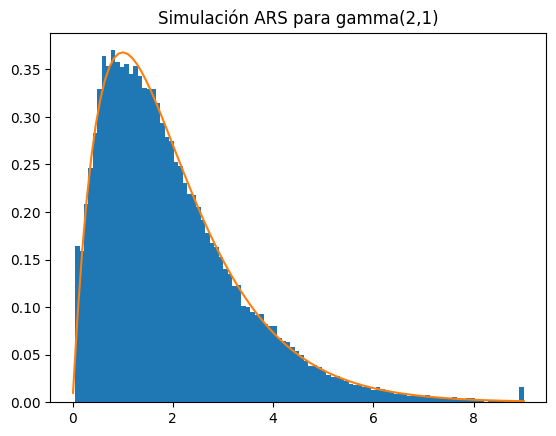
\includegraphics[width = 11 cm ]{Figures/Resultado.png} 
        \caption{Histograma para las muestras simuladas por el método ARS de la distribución gamma(2,1)}
        \label{Fig. 5.05}
    \end{figure} 

    Notemos que tenemos un buen ajuste asíntotico para la densidad objetivo. Veamos que por construcción, en los extremos tenemos masa acumulada debido a que en la inversa generalizada, al tener mallas muy finas (linspace) para valores cercanos a 1 (x grandes), no se podia encontrar un valor en la malla que no fuera menor que x. Este problema se debe a que la inversa generalizada cercana a uno puede crecer significativamente, por lo que aquellos valores $X$ de la simulación que sobrepasaran el límite establecido se agrupaban en el últimi valor del linspace.
    
    






\end{solution}


    \end{document}